\subsubsection{Agenten RTE}

Zur Umsetzung der dezentralen Steuerung werden Softwareagenten eingesetzt. Bei Software-Agenten handelt es sich um Prozesse, die lose gekoppelt 
und leicht austauschbar sind \cite[vgl.][S. 31-37]{GH:2010}. Es existieren verschiedene Definitionen eines Agenten, von denen
sich keine als Standard etablieren konnte. Die hier verwendete Definition stammt von
Brenner, Zarnekow und Wittig. Sie definieren einen Agenten als „ ... ein Softwareprogramm,
das für einen Benutzer bestimmte Aufgaben erledigen kann und dabei einen Grad an
Intelligenz besitzt, der es befähigt, seine Aufgaben in Teilen autonom durchzuführen und mit
seiner Umwelt auf sinnvolle Art und Weise zu interagieren“\cite{BZW:1998}. Die Fähigkeit von Agenten, miteinander zu kommunizieren 
und zu interagieren, ermöglicht das Erstellen eines Multiagentensystems (MAS). Ein wesentlicher Vorteil von MAS 
bzw. von verteilten Steuerungssystemen ist die Fähigkeit, dynamisch auf Veränderungen zu reagieren. Ein Beispiel für eine solche Veränderung ist der
Ausfall einer Steuerungseinheit bzw. eines Agenten. Der Ausfall einer Einheit hat nicht unbedingt zur Folge, dass das gesamte System ausfällt. 
Die restlichen Einheiten können sich eigenständig auf eine solche Veränderung einstellen und diese beim weiteren Ablauf
berücksichtigen\cite[S. 13]{Roidl:2012}. Diese Eigenschaft bringt eine ganze Reihe von Vorteilen für ein dezentral
gesteuertes Materialflusssystem mit sich.\\
Die Modellierung von agentenbasierten Systemen für industrielle Bereiche wird durch die
Entwicklung von Standards festgelegt. Diese beschreiben Modelle für die Architektur
sowie die Kommunikation zwischen Agenten. Die FIPA (Foundation of Intelligent Physical Agents) ist das Standardisierungsorgan für Agentensysteme.
Seit der Gründung 1996 in der Schweiz wurden verschiedene Standardisierungen veröffentlicht, so zum Beispiel auch die Agentenkommunikation (Agent Communication), die als FIPA/ACL (Agent Communication Language, ACL) bekannt geworden ist. Jeder Agent ist mit einem eindeutigen
Identifikationsnamen (Agent Identifier oder AID) versehen und wird im Agent Management System verwaltet\cite[S. 24]{Roidl:2012}.
Ein Verzeichnisdienst kann optional vom Directory Facilitator gestellt
werden. Die Komponenten sind über das Message Transport System (MTS) verbunden,
sodass alle Komponenten untereinander kommunizieren können\cite[S. 24]{Roidl:2012}. \\
Als Referenzmodell zur Verwaltung von Softwareagenten wurde die Softwarearchitektur der Materialflussgruppe laut den FIPA Standards aufgebaut. 
Die nächste Abbildung zeigt den Aufbau der Softwarearchitektur und ist an die AUTOSAR Softwarearchitektur angelehnt:
\begin{figure}[h!]
	\centering
		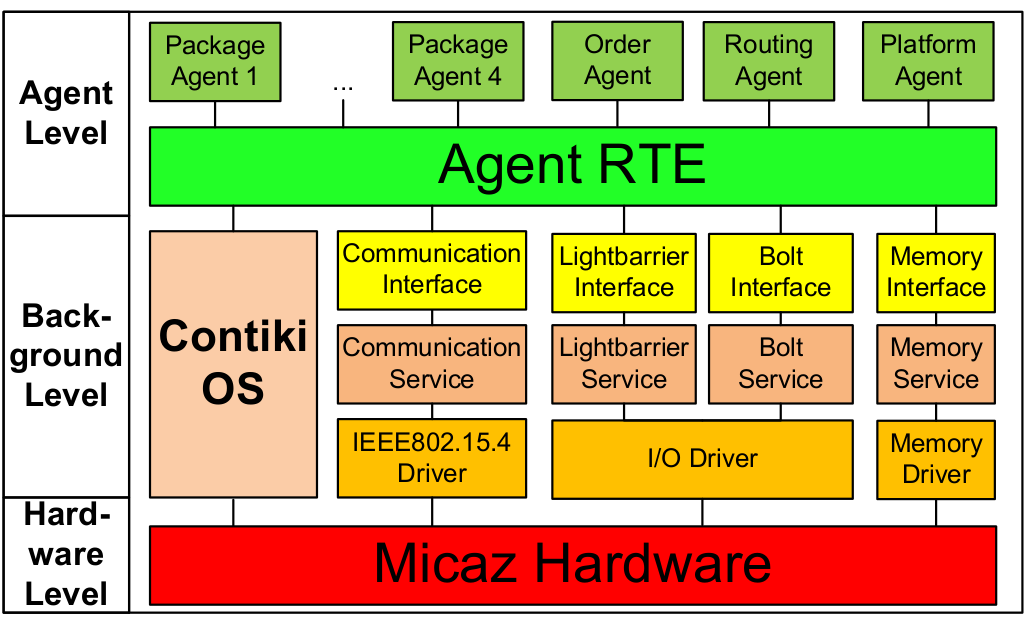
\includegraphics[width=0.9\textwidth]{ArchitekturMicazRampe.png}
	\caption{Architektur Micaz Rampe\cite{Stasch:Hahn}}
	\label{ArchitekturMicazRampe}
\end{figure}
\paragraph{Hardware Level}
Auf der Hardwareebene werden die Treiber für die Steuerung der Lichtschranke und Bolzen implementiert. Die Treiber bekommen ein
allgemeines Interface für die Agenten RTE.